\subsubsection{Base Controller}
\label{subsubsec:02psesTrajectory}

Das Fahrzeug wird tats"achlich von einem Knoten gesteuert, dessen Aufgabe darin besteht, die Stellgr"o"sen f"ur den Motor und die Lenkung zu berechnen und die verschiedenen Ziele f"ur den Rundkurs zu setzen.

\paragraph{Modelle}
Da die Lenkwinkel- und Geschwindigkeitsbefehle aus dem Navigation Stack in \texttt{m/s} und in \texttt{rad} gepublished werden, m"ussen sie zu Stellgr"o"sen umgerechnet werden. Hierf"ur werden die im Abschnitt \ref{subsec:02modellbildung} beschriebenen Geschwindigkeits- und Lenkwinkelmodelle genutzt. Diese Stellgr"o"sen werden dann als Topics f"ur die \texttt{uc\_bridge} gepublished.

\paragraph{Zielsetzung}
Damit eine Trajektorie geplant wird, muss dem Navigation Stack ein Ziel "ubergeben werden. Es bestehen mehrere M"oglichkeiten daf"ur. Entweder gibt man ein Ziel manuell in rviz vor, oder man publisht ein Ziel direkt in dem Topic \texttt{/move\_base\_simple/goal}.\\
Um den Rundkurs zu fahren, wurden mehrere Ziele entlang der Strecke gesetzt, wie in Abbildung \ref{fig:goals} dargestellt. Mithilfe eines Z"ahlers wird jedes Ziel automatisch aktiviert, sobald das Fahrzeug sich ausreichend dem vorherigen Ziel gen"ahert hat, d.h. in einer Entfernung kleiner als 1,5m.

\begin{figure}[H]
	\centering
	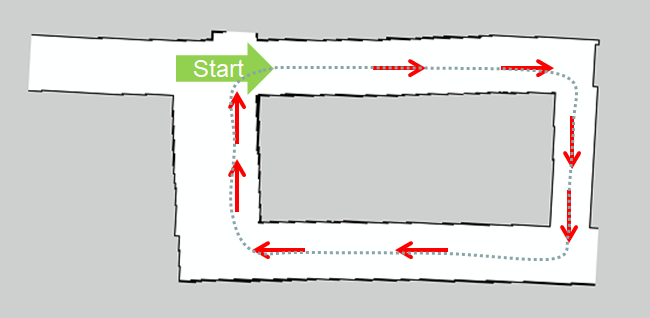
\includegraphics[width=0.8\textwidth,trim=2.4cm 0cm 0cm 1cm,clip]{pics/goals.png}
	\caption{Aufeinanderfolgenden Ziele entlang des Parcours}
	\label{fig:goals}
\end{figure}

\paragraph{Recovery Behavior}
Wie bereits im Kapitel \ref{subsubsec:02navigatinStack} (siehe Probleme) erw"ahnt, ist es m"oglich, dass der lokale Planer aufgrund der Pr"asenz von Artefakten in der Costmap keine vern"unftige Trajektorie berechnen kann. Das Auto f"ahrt dann abwechselnd r"uck- und vorw"arts, ohne einen Ausweg zu finden. Um dieses Problem zu beheben, wurde ein eigenes \emph{Recovery Behavior} implementiert, welches dieses problematische Verhalten erkennen und das Obstacle Layer in der Costmap leeren soll.\\
Diese Implementierung hat jedoch nicht funktioniert, da das richtige Layer beim Leeren der Costmap nicht gefunden werden konnte. Aus Zeitmangel konnte dieser Fehler nicht behoben werden.